\documentclass{beamer}
\usetheme{Boadilla} 
\setbeamercovered{invisible}
\setbeamertemplate{navigation symbols}{} 
%\useoutertheme{infolines} 

\usepackage[utf8]{inputenc}
\usepackage{graphicx}

\setbeamertemplate{frametitle continuation}{} 
\usepackage{subfigure}
\usepackage{caption}
\usepackage{bm}
\usepackage{epsfig}

\usepackage{amsmath}
\usepackage{xcolor,colortbl}

\usepackage{multicol}
\usepackage{wasysym}

\usepackage{hyperref}
\usepackage{float}

\usepackage{array}
\newcolumntype{L}[1]{>{\raggedright\let\newline\\\arraybackslash\hspace{0pt}}m{#1}}
\newcolumntype{C}[1]{>{\centering\let\newline\\\arraybackslash\hspace{0pt}}m{#1}}
\newcolumntype{R}[1]{>{\raggedleft\let\newline\\\arraybackslash\hspace{0pt}}m{#1}}

\usepackage[T1]{fontenc}
\usepackage{tikz}
\usetikzlibrary{shadows}

\newcommand*\keystroke[1]{%
  \tikz[baseline=(key.base)]
    \node[%
      draw,
      fill=white,
      drop shadow={shadow xshift=0.25ex,shadow yshift=-0.25ex,fill=black,opacity=0.75},
      rectangle,
      rounded corners=2pt,
      inner sep=1pt,
      line width=0.5pt,
      font=\scriptsize\sffamily
    ](key) {#1\strut}
  ;
}

% deal with spaces in absolute paths

\usepackage[space]{grffile}
\graphicspath{{C:/Users/Yered/Dropbox/Harvard/Winter 2014/CdeC/Slides/Introduction/figures/}}

\usepackage[scaled]{helvet}
\usepackage[round]{natbib}


\begin{document}
%\title[Explorando el Transcriptoma]{Explorando el Transcriptoma con Datos de Expresi\'{o}n Gen\'{e}tica}
%\author{Yered Pita-Ju\'{a}rez}
%\institute[CdeC M\'{e}rida]{}
%\date{??/??/2015}
\title[Introducción a R \& RStudio]{Explorando el Transcriptoma con Datos de Expresi\'{o}n Gen\'{e}tica\\
\vspace{0.5cm}
Introducción a R \& RStudio}
\author{Yered Pita-Ju\'{a}rez}
\institute[CdeC M\'{e}rida]{}
\date{3/1/2015}


\begin{frame}
\titlepage
\end{frame}

\begin{frame}[fragile]{Working Directory}
\begin{itemize}
\item \texttt{Working directory} es el folder en tu computadora que R está usando
\item Cuando intentes abrir un archivo, R lo buscara en el \texttt{working directory}
\item Cuando guardes un archivo desde R, lo guardará en el \texttt{working directory}
\item Antes de que empieces a trabajar, asegúrate de que el \texttt{working directory} sea el folder donde están tus datos o donde quieres guardar los resultados
\item ¿Cuál es el working directory?
\begin{verbatim}
getwd()
\end{verbatim}

\end{itemize}
\end{frame}

\begin{frame}[fragile]{Working Directory}
\begin{itemize}
\item Para cambiar el working directory desde la línea de comando usa \texttt{setwd("nombredelfolder")}. Por ejemplo
\begin{verbatim}
setwd("C:/UsuarioResignado/Aqui/Mismo/")
\end{verbatim}
\item Usa \verb=/= en lugar de \verb=\=
\item No olvides usar los apóstrofes \verb=""=
\item En RStudio\\
\texttt{Session/Set working directory}
\end{itemize}
\begin{figure}[H]
\centering
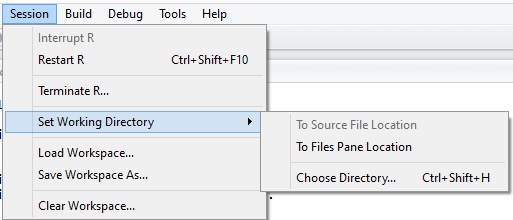
\includegraphics[scale=0.5]{rstudio_setwd.png}
\end{figure}
\end{frame}

\begin{frame}{Working Directory}
\begin{block}{Ejercicio}
\begin{itemize}
\item ¿Cuál es el \texttt{working directory}? Usa el comando \texttt{getwd()}.
\item Crea un folder llamado \texttt{CdeC} y hazlo el \texttt{working directory} usando el comando \texttt{setwd()}.
\end{itemize}
\end{block}
\begin{figure}[H]
\centering

\includegraphics[scale=0.15]{laptop.jpeg}
\end{figure}
\end{frame}

\begin{frame}[fragile]{Packages}
\begin{itemize}
\item Las funciones de R estan organizadas en \texttt{packages}
\item ¿Qué packages están instalados?
\begin{verbatim}
library()
\end{verbatim}
\item En RStudio el panel de \texttt{packages}
\begin{figure}[H]
\centering
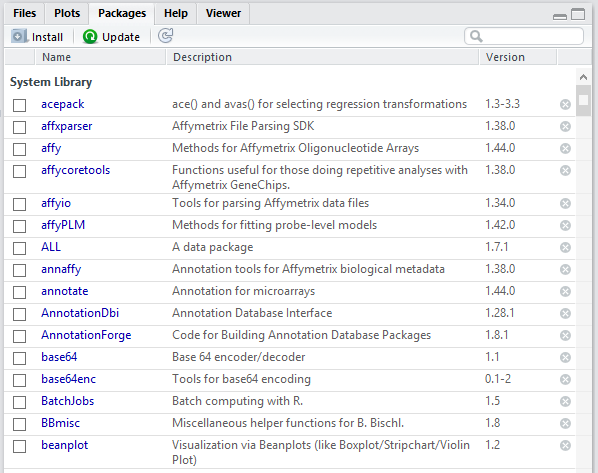
\includegraphics[scale=0.4]{rstudio_pkg_panel.png}
\end{figure}
\end{itemize}
\end{frame}

\begin{frame}[fragile]{Packages}
\begin{itemize}
\item Para instalar un package
\begin{verbatim}
install.packages("nombredelpackage")
\end{verbatim}
\item En RStudio
\begin{figure}[H]
\centering
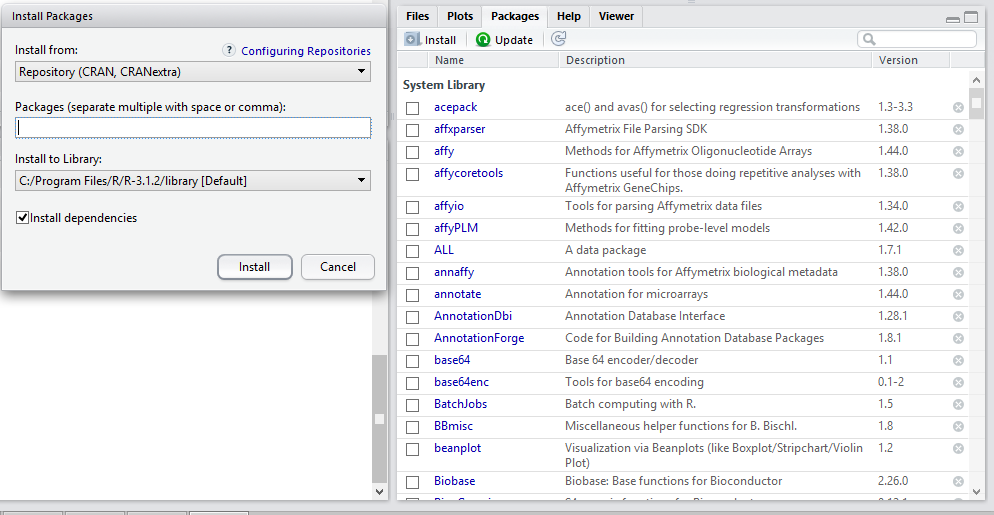
\includegraphics[scale=0.35]{rstudio_install_pkg.png}
\end{figure}
\end{itemize}
\end{frame}

\begin{frame}[fragile]{Packages}
\begin{itemize}
\item Para cargar un \texttt{package} ya instalado
\begin{verbatim}
library("nombredelpackage")
\end{verbatim}
\item En RStudio selecciona el \texttt{package} desde el panel 
\begin{figure}[H]
\centering
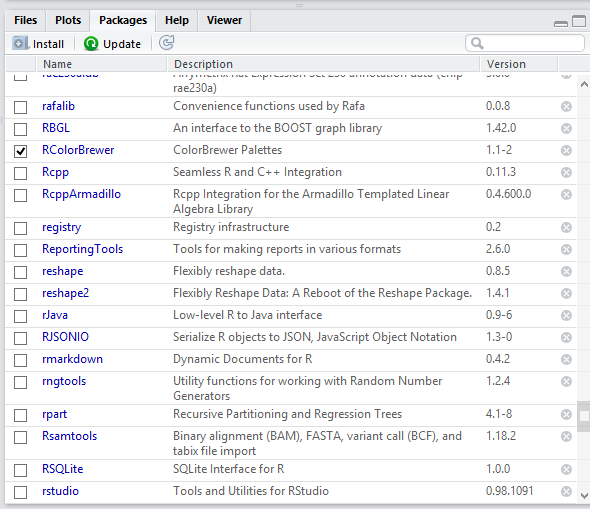
\includegraphics[scale=0.35]{rstudio_load_pkg.png}
\end{figure}
\end{itemize}
\end{frame}

\begin{frame}[fragile]{Packages}
\begin{block}{Ejercicio}
\begin{itemize}
\item Instala el paquete \texttt{RColorBrewer}
\item Carga el  paquete \texttt{RColorBrewer}
%\item Si lo hiciste correctamente, el siguiente comando debe generar un gráfico
%\begin{verbatim}
%display.brewer.pal(7,"Accent")
%\end{verbatim}
\end{itemize}
\end{block}
\begin{figure}[H]
\centering

\includegraphics[scale=0.15]{laptop.jpeg}
\end{figure}
\end{frame}

\begin{frame}[fragile]{Packages}
\begin{block}{Ejercicio}
\begin{itemize}
%\item Instala el paquete \texttt{RColorBrewer}
%\item Carga el  paquete \texttt{RColorBrewer}
\item Si lo hiciste correctamente, el siguiente comando debe generar un gráfico
\begin{verbatim}
display.brewer.pal(7,"Accent")
\end{verbatim}
\end{itemize}
\end{block}
\begin{figure}[H]
\centering
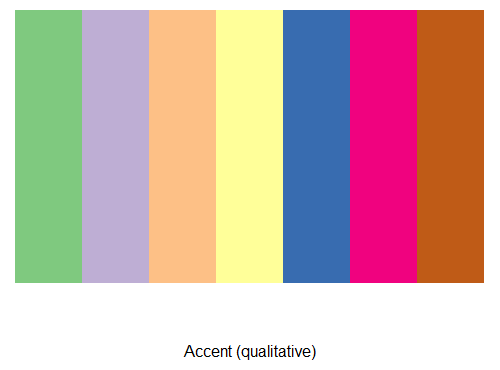
\includegraphics[scale=0.45]{rcolorbrewer_ex.png}
\end{figure}
\end{frame}

\begin{frame}[fragile]{Comandos}
\begin{itemize}
\item R puede ser usado como una calculadora
\item Escribe la ecuación despues de \verb=>= , y presiona \texttt{enter}
\begin{verbatim}
> 10^2 + 36
\end{verbatim}
\item R dará la respuesta
\begin{verbatim}
[1] 136
\end{verbatim}
\end{itemize}
\begin{figure}
\centering
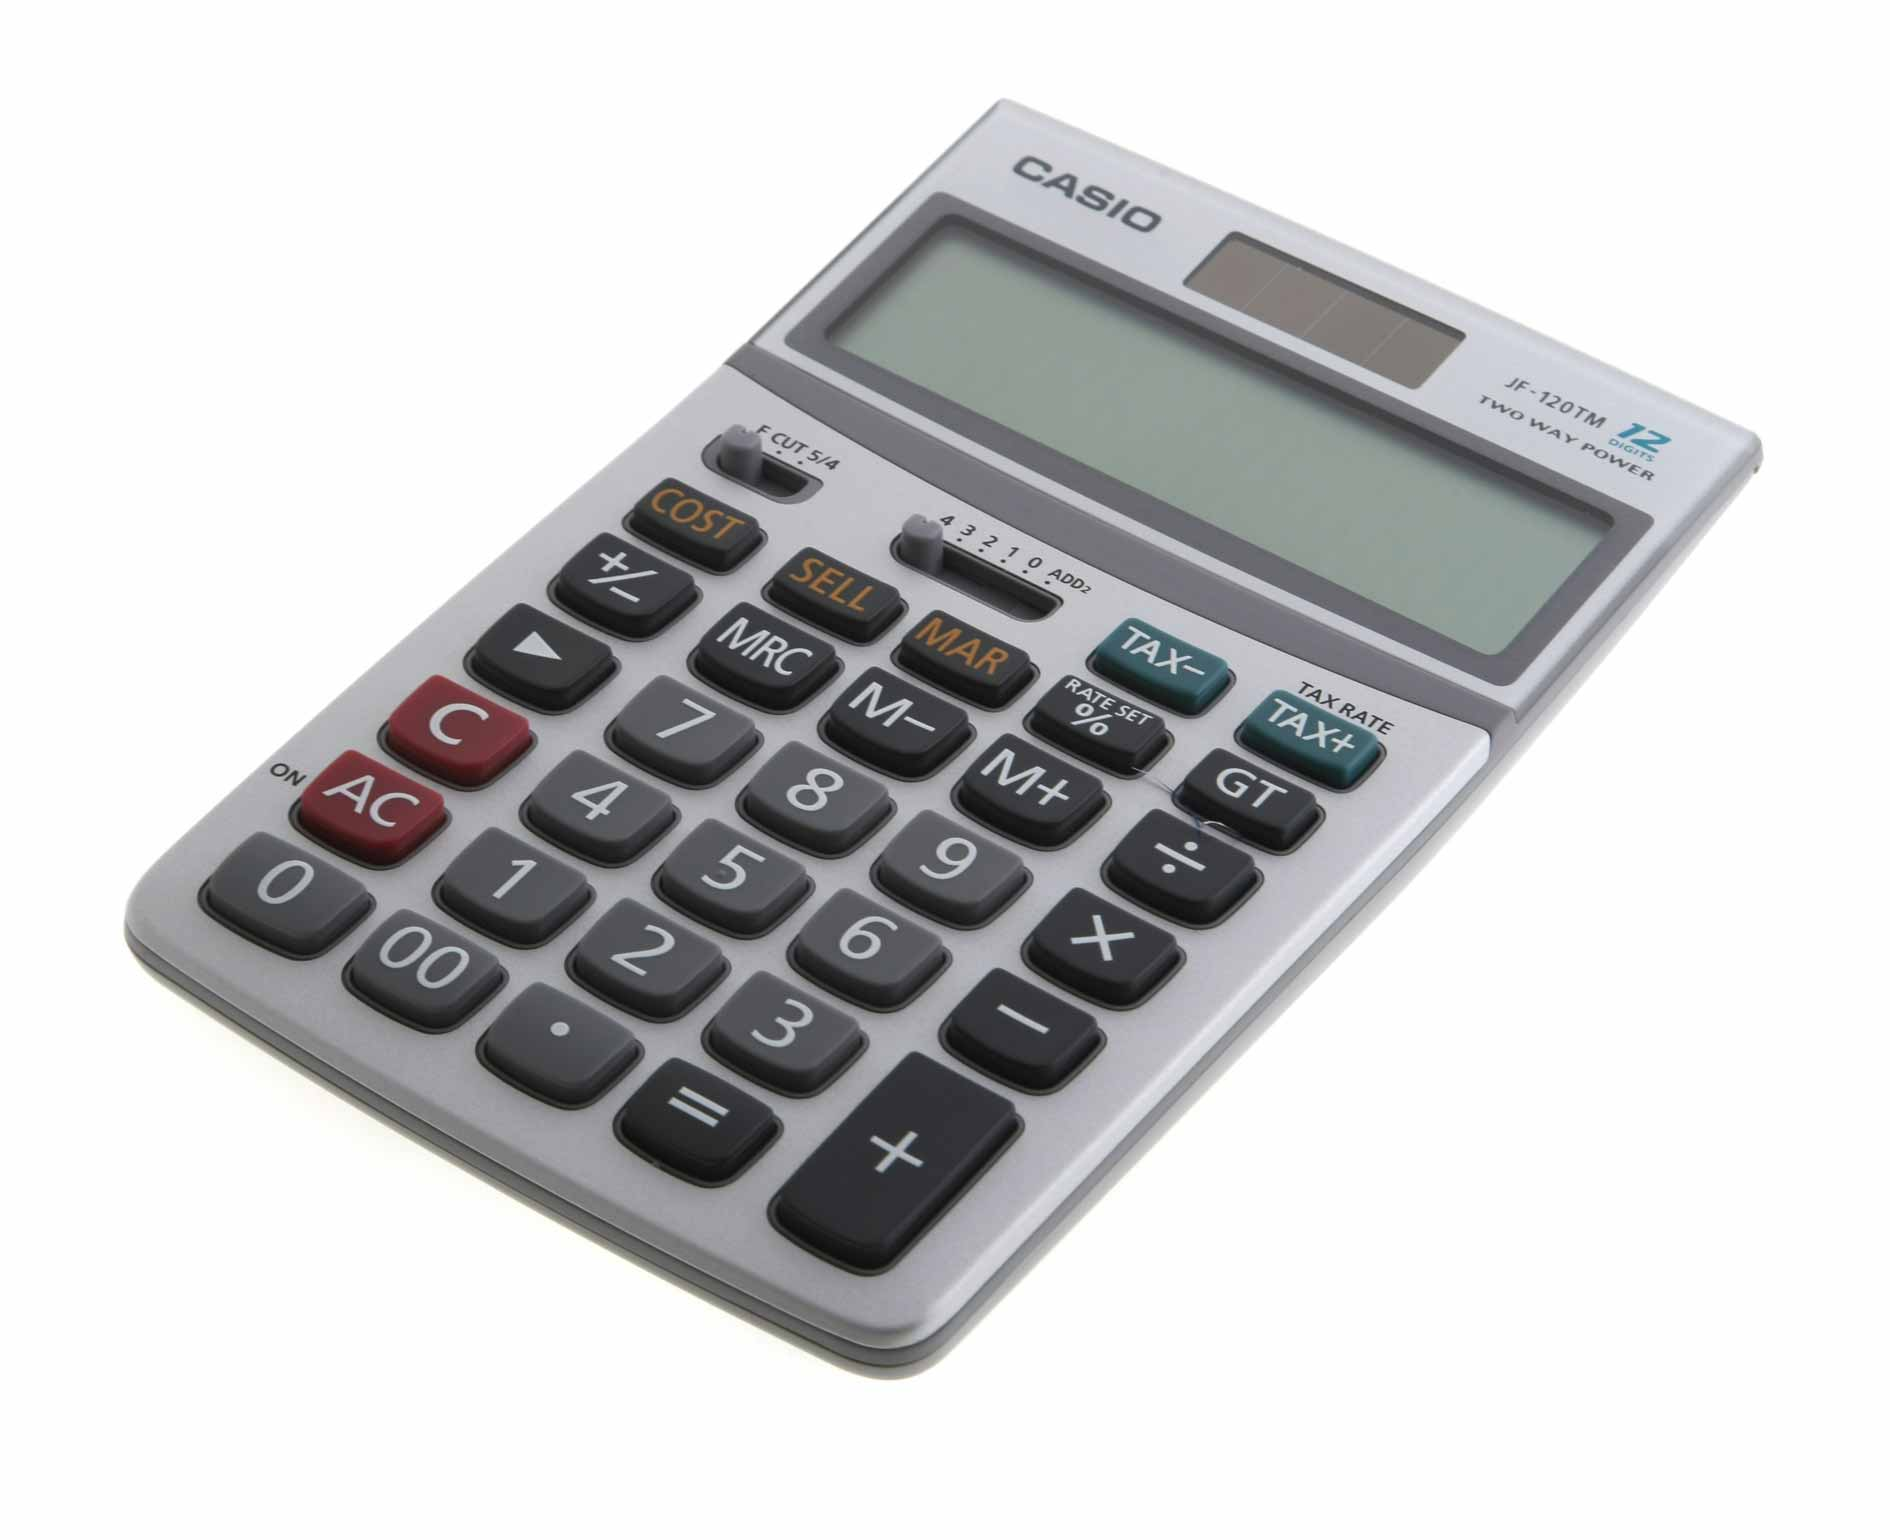
\includegraphics[scale=0.08]{calculator-01.jpg}
\end{figure}
\end{frame}

\begin{frame}[fragile]{Comandos}
\begin{block}{Ejercicio}
Calcula la diferencia entre el 2014 y el año en el que empezaste la carrera, divide este número por la diferencia entre el 2014 y el año que naciste. Multiplica este número por 100 para obtener el porcentaje de tu vida que has pasado en la univerisdad.
\end{block}
\begin{figure}[H]
\centering

\includegraphics[scale=0.5]{billy_madison.jpg}
\end{figure}
\end{frame}


\begin{frame}[fragile]{Workspace}
\begin{itemize}
\item Puedes asignar un número a una variable
\item Para crear una variable 
\begin{verbatim}
> a <- 4
\end{verbatim}
o
\begin{verbatim}
> a = 4
\end{verbatim}
\item En el panel de workspace aparece la variable \verb=a=
\item Para ver el valor asignado a esta variable
\begin{verbatim}
> a
[1] 4
\end{verbatim}
\end{itemize}
\end{frame}

\begin{frame}[fragile]{Workspace}
\begin{itemize}
\item También, puedes usarla para hacer cálculos
\begin{verbatim}
> a * 5
[1] 20
\end{verbatim}
\item Si vuelves a asignarle un valor a la variable, se pierde el valor que tenía asignado previamente
\begin{verbatim}
> a = a * 5
> a
[1] 20
\end{verbatim}
\item R es un lenguaje sensible a mayúsculas: \verb=A= y \verb=a= son dos símbolos diferentes
\item Los nombres de las variables no pueden empezar con un número
\end{itemize}
\end{frame}

\begin{frame}[fragile]{Workspace}
\begin{itemize}
\item Para ver que objectos están en la memoria
\begin{verbatim}
objects()
\end{verbatim}
\item En RStudio: en el panel de \verb=workspace=
\item Para eliminar un objecto de la memoria
\begin{verbatim}
rm(nombreobjeto)
\end{verbatim}
\item Para eliminar todos los objectos de la memoria en R
\begin{verbatim}
rm(list=ls())
\end{verbatim}
\item En RStudio usa el botón de \verb=clear= en el panel \verb=workspace=
\end{itemize}
\end{frame}

\begin{frame}[fragile]{Workspace}
\begin{block}{Ejercicio}
Repite el ejercicio anterior usando varias variables para calcular el porcentaje de tu vida que has pasado en la universidad
\end{block}
\begin{figure}[H]
\centering

\includegraphics[scale=0.5]{billy_madison.jpg}
\end{figure}
\end{frame}
%

\begin{frame}[fragile]{Workspace}
\begin{block}{Ejercicio}
\begin{itemize}
\item Elimina todas los objectos de la memoria de R
\item Crea las siguientes variables: $a=1,b=2,c=3$
\item Usa R para calcular $a+b+c$
\item Elimina la variable $b$
\item Repite la suma anterior, ¿cuál es el mensaje de error?
\end{itemize}
\end{block}
\begin{figure}[H]
\centering

\includegraphics[scale=0.14]{laptop.jpeg}
\end{figure}
\end{frame}

\begin{frame}[fragile]{Escalares, Vectores y Matrices}
\begin{itemize}
\item Los valores numéricos en R están organizados en 
\begin{itemize}
\item escalares 
\item vectores
\item matrices
\end{itemize}
\item Las variables que definimos anteriormente fueron escalares
\item Para definir un vector necesitamos la function \verb=c=
\begin{verbatim}
b=c(3,4,5)
\end{verbatim}
\end{itemize}
\end{frame}

\begin{frame}[fragile]{Funciones}
\begin{itemize}
\item Para calcular el promedio de los elementos del vector \verb=b=
\begin{verbatim}
> (3+4+5)/3
\end{verbatim}
\item Para vectores mas largos, esto no es ideal
\item Funciones: operaciones de uso frecuente 
\item Para calcular el promedio
\begin{verbatim}
> mean(x=b)
\end{verbatim}
\item Dentro del paréntesis están los argumentos de la función
\item No siempre es necesario incluir los nombres de los argumentos
\begin{verbatim}
> mean(b)
\end{verbatim}
\end{itemize}
\end{frame}

\begin{frame}[fragile]{Funciones}
\begin{block}{Ejercicio}
\begin{itemize}
\item Calcula la edad promedio de la clase.
\item Primero preguntale a tus compañer@s su edad, y crea un vector para guardar las edades de la clase
\item Usa la función \verb=sum= para calcular el promedio
\item Usa la función \verb=mean= para calcular el promedio
\end{itemize}
\end{block}
\begin{figure}[H]
\centering

\includegraphics[scale=0.13]{laptop.jpeg}
\end{figure}
\end{frame}

\begin{frame}[fragile]{Funciones}
\begin{itemize}
\item \verb=rnorm= es una función estándar de R para generar números aleatorios de la distribución normal
\begin{verbatim}
> rnorm(10)
[1] -0.949 1.342 -0.474 0.403
[5] -0.091 -0.379 1.015 0.740
[9] -0.639 0.950
\end{verbatim}
\item la primera línea contiene el comando
\item Las líneas 2-4 contienen los resultados: un vector con 10 números aleatorios
\item ¿Cuál es el comando?
\item ¿Cuál es el argumento?
\item También podemos usar 
\begin{verbatim}
rnorm(n=10)
\end{verbatim}
\end{itemize}
\end{frame}

\begin{frame}[fragile]{Funciones}
\begin{itemize}
\item Usa \keystroke{\hspace{0.1cm}$\uparrow$\hspace{0.1cm}} para acceder a comandos usados anteriormente
\item En RStudio, usa el panel de \verb=history=
\begin{figure}[H]
\centering
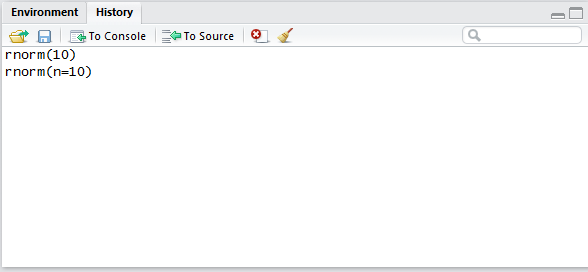
\includegraphics[scale=0.35]{rstudio_history.png}
\end{figure}
\end{itemize}
\end{frame}


\begin{frame}[fragile]{Funciones}
\begin{itemize}
\item Para generar 10 números aleatorios de una distribución normal con media 1.2 y desviación estándar de 3.4 
\begin{verbatim}
> rnorm(10, mean=1.2, sd=3.4)
\end{verbatim}
\item La función \verb=rnorm= tiene varios argumentos
\item Solo requerimos un argumento, \verb=n=, para usar \verb=rnorm=
\item Los demás argumentos son opcionales, y R tienes valores asignados a ellos por default
\item En RStudio presiona \keystroke{Tab\hspace{0.5cm}} despues de \verb=rnorm(= para ver los argumentos de la función.
\begin{figure}[H]
\centering
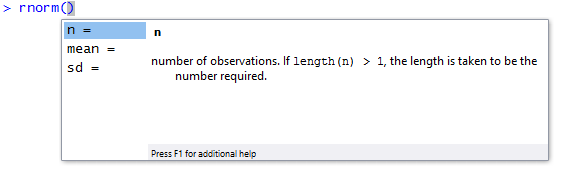
\includegraphics[scale=0.45]{rstudio_tab_args.png}
\end{figure}
\end{itemize}
\end{frame}

\begin{frame}[fragile]{Gráficas}
\begin{itemize}
\item R tiene la capacidad para generar gráficas
\item Un ejemplo muy simple
\begin{verbatim}
> x = rnorm(100)
> plot(x)
\end{verbatim}
\item Primero generamos 100 números aleatorios de una distribución normal
\item En la segunda línea graficamos estos valores
\end{itemize}
\end{frame}

\begin{frame}[fragile]{Gráficas}
\begin{block}{Ejercicio}
\begin{itemize}
\item Las funciones \verb=hist= y \verb=boxplot= son muy útiles para ver la distribución de una variable
\item Usa las funciones \verb=hist= y \verb=boxplot= para generar gráficas acerca de la edad de la clase
\end{itemize}
\end{block}
\begin{figure}[H]
\centering

\includegraphics[scale=0.15]{laptop.jpeg}
\end{figure}
\end{frame}


\begin{frame}[fragile]{Ayuda}
\begin{itemize}
\item R incluye archivos de ayuda para sus funciones
\begin{verbatim}
> help(rnorm)
\end{verbatim}
\begin{figure}[H]
\centering
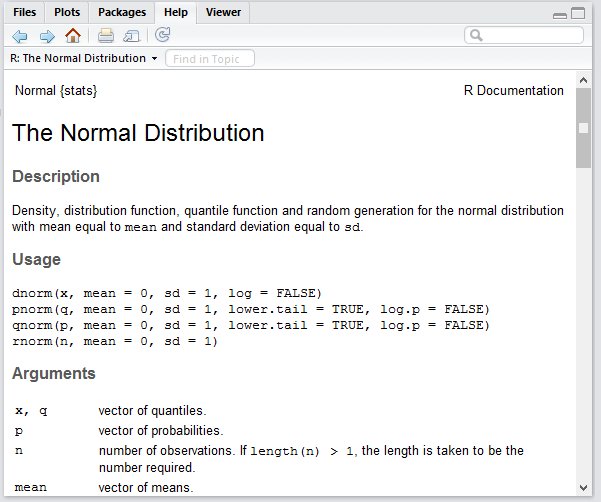
\includegraphics[scale=0.35]{rstudio_rnorm_help.png}
\end{figure}
\item La ayuda da una descripción de la función y de sus argumentos, así como de los valores default
\item Algunas funciones incluyen ejemplos de su uso
\begin{verbatim}
> example(rnorm)
\end{verbatim}
\end{itemize}
\end{frame}


\begin{frame}[fragile]{Ayuda}
\begin{itemize}
\item Los archivos de ayuda para una función se pueden acceder también usando
\begin{verbatim}
?nombrefuncion
\end{verbatim}
\item Por ejemplo
\begin{verbatim}
?rnorm
\end{verbatim}
\item Para buscar dentro de los archivos de ayuda podemos usar
\begin{verbatim}
??tema
\end{verbatim}
o
\begin{verbatim}
help.search("tema")
\end{verbatim}
\end{itemize}
\end{frame}


\begin{frame}[fragile]{Ayuda}
\begin{itemize}
\item El manual de ayuda se puede acceder mediante
\begin{verbatim}
> help.start()
\end{verbatim}
\end{itemize}
\begin{figure}[H]
\centering
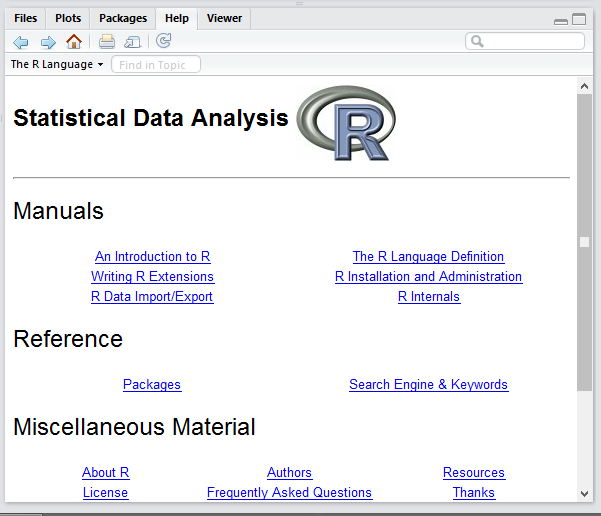
\includegraphics[scale=0.35]{r_help_menu.png}
\end{figure}
\end{frame}

\begin{frame}[fragile]{Ayuda}
\begin{block}{Ejercicio}
\begin{itemize}
\item Busca los archivos de ayuda relacionados a \texttt{hypergeometric}
\item ¿Qué función encontraste?
\item ¿Qué ejemplos hay disponibles?
\end{itemize}
\end{block}
\begin{figure}[H]
\centering

\includegraphics[scale=0.15]{laptop.jpeg}
\end{figure}
\end{frame}


\begin{frame}[fragile]{Scripts}
\begin{itemize}
\item R es un lenguaje de línea de comando
\item Scripts: archivos para guardar comandos 
\item Por lo general el nombre es
\begin{verbatim}
miscript.R
\end{verbatim}
\item En RStudio, en el panel script puedes correr líneas de comando seleccionandolas y después presionando \keystroke{CTRL} $+$ \keystroke{ENTER\hspace{0.15cm}} o presionando el botón de \texttt{run}
\begin{figure}[H]
\centering
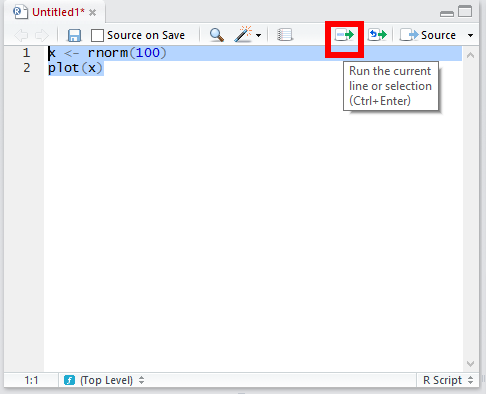
\includegraphics[scale=0.45]{rstudio_run_script}
\end{figure}
\item Desde la consola, puedes correr un script usando
\begin{verbatim}
> source("miscript.R")
\end{verbatim}
\end{itemize}
\end{frame}


\begin{frame}{Scripts}
\begin{block}{Ejercicio}
Crea un script llamado miprimerscript.R que genere y grafique 100 números aleatorios 
\end{block}
\begin{figure}[H]
\centering

\includegraphics[scale=0.15]{laptop.jpeg}
\end{figure}
\end{frame}

%\begin{frame}[fragile]{}
%\end{frame}

%
%
%\begin[fragile]{frame}{}
%\begin{block}{Ejercicio}

%\end{block}
%\begin{figure}[H]
%\centering
%
\includegraphics[scale=0.15]{laptop.jpeg}
%\end{figure}
%\end{frame}
%
%




\end{document} 

